% Options for packages loaded elsewhere
\PassOptionsToPackage{unicode}{hyperref}
\PassOptionsToPackage{hyphens}{url}
%
\documentclass[
]{book}
\usepackage{lmodern}
\usepackage{amssymb,amsmath}
\usepackage{ifxetex,ifluatex}
\ifnum 0\ifxetex 1\fi\ifluatex 1\fi=0 % if pdftex
  \usepackage[T1]{fontenc}
  \usepackage[utf8]{inputenc}
  \usepackage{textcomp} % provide euro and other symbols
\else % if luatex or xetex
  \usepackage{unicode-math}
  \defaultfontfeatures{Scale=MatchLowercase}
  \defaultfontfeatures[\rmfamily]{Ligatures=TeX,Scale=1}
\fi
% Use upquote if available, for straight quotes in verbatim environments
\IfFileExists{upquote.sty}{\usepackage{upquote}}{}
\IfFileExists{microtype.sty}{% use microtype if available
  \usepackage[]{microtype}
  \UseMicrotypeSet[protrusion]{basicmath} % disable protrusion for tt fonts
}{}
\makeatletter
\@ifundefined{KOMAClassName}{% if non-KOMA class
  \IfFileExists{parskip.sty}{%
    \usepackage{parskip}
  }{% else
    \setlength{\parindent}{0pt}
    \setlength{\parskip}{6pt plus 2pt minus 1pt}}
}{% if KOMA class
  \KOMAoptions{parskip=half}}
\makeatother
\usepackage{xcolor}
\IfFileExists{xurl.sty}{\usepackage{xurl}}{} % add URL line breaks if available
\IfFileExists{bookmark.sty}{\usepackage{bookmark}}{\usepackage{hyperref}}
\hypersetup{
  pdftitle={Restoration of Submerged Aquatic Vegetation},
  pdfauthor={Kate Sinnott},
  hidelinks,
  pdfcreator={LaTeX via pandoc}}
\urlstyle{same} % disable monospaced font for URLs
\usepackage{color}
\usepackage{fancyvrb}
\newcommand{\VerbBar}{|}
\newcommand{\VERB}{\Verb[commandchars=\\\{\}]}
\DefineVerbatimEnvironment{Highlighting}{Verbatim}{commandchars=\\\{\}}
% Add ',fontsize=\small' for more characters per line
\usepackage{framed}
\definecolor{shadecolor}{RGB}{248,248,248}
\newenvironment{Shaded}{\begin{snugshade}}{\end{snugshade}}
\newcommand{\AlertTok}[1]{\textcolor[rgb]{0.94,0.16,0.16}{#1}}
\newcommand{\AnnotationTok}[1]{\textcolor[rgb]{0.56,0.35,0.01}{\textbf{\textit{#1}}}}
\newcommand{\AttributeTok}[1]{\textcolor[rgb]{0.77,0.63,0.00}{#1}}
\newcommand{\BaseNTok}[1]{\textcolor[rgb]{0.00,0.00,0.81}{#1}}
\newcommand{\BuiltInTok}[1]{#1}
\newcommand{\CharTok}[1]{\textcolor[rgb]{0.31,0.60,0.02}{#1}}
\newcommand{\CommentTok}[1]{\textcolor[rgb]{0.56,0.35,0.01}{\textit{#1}}}
\newcommand{\CommentVarTok}[1]{\textcolor[rgb]{0.56,0.35,0.01}{\textbf{\textit{#1}}}}
\newcommand{\ConstantTok}[1]{\textcolor[rgb]{0.00,0.00,0.00}{#1}}
\newcommand{\ControlFlowTok}[1]{\textcolor[rgb]{0.13,0.29,0.53}{\textbf{#1}}}
\newcommand{\DataTypeTok}[1]{\textcolor[rgb]{0.13,0.29,0.53}{#1}}
\newcommand{\DecValTok}[1]{\textcolor[rgb]{0.00,0.00,0.81}{#1}}
\newcommand{\DocumentationTok}[1]{\textcolor[rgb]{0.56,0.35,0.01}{\textbf{\textit{#1}}}}
\newcommand{\ErrorTok}[1]{\textcolor[rgb]{0.64,0.00,0.00}{\textbf{#1}}}
\newcommand{\ExtensionTok}[1]{#1}
\newcommand{\FloatTok}[1]{\textcolor[rgb]{0.00,0.00,0.81}{#1}}
\newcommand{\FunctionTok}[1]{\textcolor[rgb]{0.00,0.00,0.00}{#1}}
\newcommand{\ImportTok}[1]{#1}
\newcommand{\InformationTok}[1]{\textcolor[rgb]{0.56,0.35,0.01}{\textbf{\textit{#1}}}}
\newcommand{\KeywordTok}[1]{\textcolor[rgb]{0.13,0.29,0.53}{\textbf{#1}}}
\newcommand{\NormalTok}[1]{#1}
\newcommand{\OperatorTok}[1]{\textcolor[rgb]{0.81,0.36,0.00}{\textbf{#1}}}
\newcommand{\OtherTok}[1]{\textcolor[rgb]{0.56,0.35,0.01}{#1}}
\newcommand{\PreprocessorTok}[1]{\textcolor[rgb]{0.56,0.35,0.01}{\textit{#1}}}
\newcommand{\RegionMarkerTok}[1]{#1}
\newcommand{\SpecialCharTok}[1]{\textcolor[rgb]{0.00,0.00,0.00}{#1}}
\newcommand{\SpecialStringTok}[1]{\textcolor[rgb]{0.31,0.60,0.02}{#1}}
\newcommand{\StringTok}[1]{\textcolor[rgb]{0.31,0.60,0.02}{#1}}
\newcommand{\VariableTok}[1]{\textcolor[rgb]{0.00,0.00,0.00}{#1}}
\newcommand{\VerbatimStringTok}[1]{\textcolor[rgb]{0.31,0.60,0.02}{#1}}
\newcommand{\WarningTok}[1]{\textcolor[rgb]{0.56,0.35,0.01}{\textbf{\textit{#1}}}}
\usepackage{longtable,booktabs}
% Correct order of tables after \paragraph or \subparagraph
\usepackage{etoolbox}
\makeatletter
\patchcmd\longtable{\par}{\if@noskipsec\mbox{}\fi\par}{}{}
\makeatother
% Allow footnotes in longtable head/foot
\IfFileExists{footnotehyper.sty}{\usepackage{footnotehyper}}{\usepackage{footnote}}
\makesavenoteenv{longtable}
\usepackage{graphicx,grffile}
\makeatletter
\def\maxwidth{\ifdim\Gin@nat@width>\linewidth\linewidth\else\Gin@nat@width\fi}
\def\maxheight{\ifdim\Gin@nat@height>\textheight\textheight\else\Gin@nat@height\fi}
\makeatother
% Scale images if necessary, so that they will not overflow the page
% margins by default, and it is still possible to overwrite the defaults
% using explicit options in \includegraphics[width, height, ...]{}
\setkeys{Gin}{width=\maxwidth,height=\maxheight,keepaspectratio}
% Set default figure placement to htbp
\makeatletter
\def\fps@figure{htbp}
\makeatother
\setlength{\emergencystretch}{3em} % prevent overfull lines
\providecommand{\tightlist}{%
  \setlength{\itemsep}{0pt}\setlength{\parskip}{0pt}}
\setcounter{secnumdepth}{5}
\usepackage{booktabs}
\usepackage[]{natbib}
\bibliographystyle{apalike}

\title{Restoration of Submerged Aquatic Vegetation}
\author{Kate Sinnott}
\date{2021-03-08}

\begin{document}
\maketitle

{
\setcounter{tocdepth}{1}
\tableofcontents
}
\hypertarget{project-introduction}{%
\chapter{Project Introduction}\label{project-introduction}}

\hypertarget{database-structure}{%
\chapter{Database Structure}\label{database-structure}}

\hypertarget{rsqlite-package}{%
\section{RSQLite Package}\label{rsqlite-package}}

The R package DBI (database interface) allows R to interface with SQLite. So first,
we install DBI:

\begin{Shaded}
\begin{Highlighting}[]
\KeywordTok{library}\NormalTok{(DBI)}
\end{Highlighting}
\end{Shaded}

\hypertarget{establishing-a-database-connection}{%
\section{Establishing a database connection}\label{establishing-a-database-connection}}

I have already created a database for my SAV restoration project in SQLite,
so now I need to connect to that database using \texttt{dbConnect}.

\begin{Shaded}
\begin{Highlighting}[]
\NormalTok{restoration_db <-}\StringTok{ }\KeywordTok{dbConnect}\NormalTok{(RSQLite}\OperatorTok{::}\KeywordTok{SQLite}\NormalTok{(),}\StringTok{"/Users/katesinnott/Desktop/WILD_6900/SAV_restoration/SAV_restoration.db"}\NormalTok{)}
\end{Highlighting}
\end{Shaded}

\hypertarget{building-database-tables}{%
\section{Building database tables}\label{building-database-tables}}

Now I need to start creating my database tables. To do this I use \texttt{dbExecute}, then
just type in the query like I would in SQLite. This is the database structure I will
be building:

\begin{figure}

{\centering 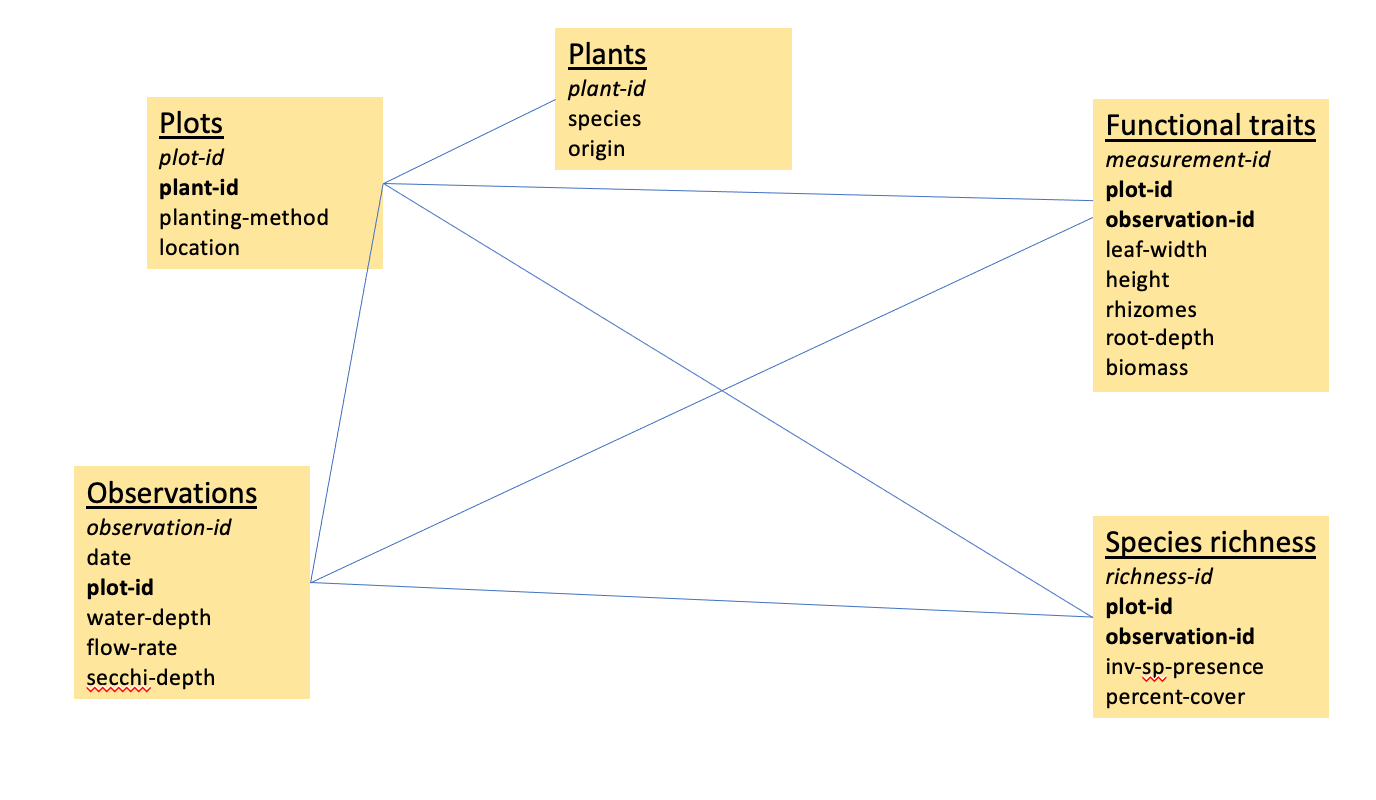
\includegraphics[width=1\linewidth]{/Users/katesinnott/Desktop/WILD_6900/SAV_restoration/Screen Shot 2021-03-01 at 7.28.09 PM} 

}

\caption{Database diagram}\label{fig:diagram}
\end{figure}

\hypertarget{table-1-plants}{%
\subsection{Table 1: Plants}\label{table-1-plants}}

I started with this table because it doesn't reference foreign keys from other tables. This table includes information I will need to reference specific plant populations -
specifically, the species and the collection locations.

\begin{Shaded}
\begin{Highlighting}[]
\KeywordTok{dbExecute}\NormalTok{(restoration_db, }\StringTok{"CREATE TABLE plants (}
\StringTok{          plant_id varchar(5) NOT NULL PRIMARY KEY,}
\StringTok{          planting_method char(9),}
\StringTok{          species varchar(6),}
\StringTok{          origin varchar(4)}
\StringTok{          );"}\NormalTok{)}
\end{Highlighting}
\end{Shaded}

\hypertarget{table-2-plots}{%
\subsection{Table 2: Plots}\label{table-2-plots}}

This table includes static information about different plots where the plants will be introduced. The foreign key is the plant\_id, which references the Plants table. Other attributes are the planting method used and the location of the plots.

\begin{Shaded}
\begin{Highlighting}[]
\KeywordTok{dbExecute}\NormalTok{(restoration_db, }\StringTok{"CREATE TABLE plots (}
\StringTok{          plot_id varchar(5) NOT NULL PRIMARY KEY,}
\StringTok{          planting_method char(9),}
\StringTok{          location varchar(6), }
\StringTok{          FOREIGN KEY (plant_id) REFERENCES plants(plant_id)}
\StringTok{          );"}\NormalTok{)}
\end{Highlighting}
\end{Shaded}

\hypertarget{table-3-observations}{%
\subsection{Table 3: Observations}\label{table-3-observations}}

The observations table includes the data collected at each plot on different collecting days. The foreign key is the plot\_id column, which references the Plots table. This data is not static. In addition to date, attributes included are water depth, flow rate, and Secchi depth, which very variable in the restoration system.

\begin{Shaded}
\begin{Highlighting}[]
\KeywordTok{dbExecute}\NormalTok{(restoration_db, }\StringTok{"CREATE TABLE observations (}
\StringTok{          observation_id varchar(10) NOT NULL PRIMARY KEY,}
\StringTok{          date text,}
\StringTok{          plot_id varchar(5), }
\StringTok{          water_depth float, }
\StringTok{          flow_rate float,}
\StringTok{          secchi_depth float,}
\StringTok{          FOREIGN KEY (plot_id) REFERENCES plots(plot_id)}
\StringTok{          );"}\NormalTok{)}
\end{Highlighting}
\end{Shaded}

\hypertarget{table-4-functional-traits}{%
\subsection{Table 4: Functional Traits}\label{table-4-functional-traits}}

This is where measurements of specific plants are recorded. This will be used to determine the success of the different plots. There are two foreign keys: plot\_id and observation\_id. Functional traits measured are leaf wisth, height, rhizomes, root depth, and shoot biomass.

\begin{Shaded}
\begin{Highlighting}[]
\KeywordTok{dbExecute}\NormalTok{(restoration_db, }\StringTok{"CREATE TABLE functional_traits (}
\StringTok{          measurement_id varchar(5) NOT NULL PRIMARY KEY,}
\StringTok{          plant_id varchar(5),}
\StringTok{          observation_id varchar(10), }
\StringTok{          leaf_width float, }
\StringTok{          height float, }
\StringTok{          rhizomes float, }
\StringTok{          root_depth float,}
\StringTok{          biomass float, }
\StringTok{          FOREIGN KEY (plot_id) REFERENCES plots(plot_id),}
\StringTok{          FOREIGN KEY (observation_id) REFERENCES observations(observation_id)}
\StringTok{          );"}\NormalTok{)}
\end{Highlighting}
\end{Shaded}

\hypertarget{table-5-species-richness}{%
\subsection{Table 5: Species richness}\label{table-5-species-richness}}

This table includes measurements to evaluate species richness. It has two foreign keys: observation and plot identifications. Attributes measured are presence of invasive species and percent cover of each species.

\begin{Shaded}
\begin{Highlighting}[]
\KeywordTok{dbExecute}\NormalTok{(restoration_db, }\StringTok{"CREATE TABLE species_richness (}
\StringTok{          richness_id varchar(10) NOT NULL PRIMARY KEY,}
\StringTok{          plot_id varchar(5),}
\StringTok{          observation_id varchar(10),}
\StringTok{          inv_sp_presence_score integer, }
\StringTok{          percent_cover integer,}
\StringTok{          FOREIGN KEY (plot_id) REFERENCES plots(plot_id),}
\StringTok{          FOREIGN KEY (observation_id) REFERENCES observations(observation_id)}
\StringTok{          );"}\NormalTok{)}
\end{Highlighting}
\end{Shaded}

  \bibliography{book.bib,packages.bib}

\end{document}
